% LaTeX Poster vim:ts=2 sw=2
% 
\documentclass[final,xcolor={svgnames}]{beamer}

\newcommand{\leftlogo}{
\includegraphics[height=1.5in]{figures/stanford.pdf}}
%\newcommand{\rightlogo}{{\Huge$\mathbb{P}\lambda$}}
\newcommand{\leftfooter}{$\mathbb{P}\lambda$ at Stanford University}
\newcommand{\rightfooter}{\texttt{chaganty@cs.stanford.edu, pliang@cs.stanford.edu}}
\mode<presentation>{\usetheme{I6pd2}}

\usepackage{grffile}
\usepackage[english]{babel}
\usepackage[latin1]{inputenc}
\usepackage{amsmath,amsthm, amssymb, latexsym}
\usepackage{algorithm,algorithmic}

\boldmath
\usepackage{graphicx}
\usepackage[orientation=portrait,size=a2,scale=1.4]{beamerposter}
% change list indention level
% \setdefaultleftmargin{3em}{}{}{}{}{}
%\usepackage{snapshot} % will write a .dep file with all dependencies, allows for easy bundling

\usepackage{array,booktabs,tabularx}
\newcolumntype{Z}{>{\centering\arraybackslash}X} % centered tabularx columns


%\listfiles

%%%%%%%%%%%%%%%%%%%%%%%%%%%%%%%%%%%%%%%%%%%%%%%%%%%%%%%%%%%%%%%%%%%%%%%%%%%%%%%%%%%%%%
\graphicspath{{figures/}}
\usepackage{scabby}

\newcommand<>{\drawgen}[1]{%
  \uncover#2{
    \point{start-gen}{#1}
    \node[style=node] (h) at (start-gen) {};
    \node[left=0.1cm of h] {$h$};
    \node[style=node,fill=green!70,below=1cm of h] (x) {};
    \node[left=0.1cm of x] {$x$};
    \draw[-latex] (h) -- (x);
  }
}

\newcommand<>{\drawdisc}[1]{%
  \uncover#2{
    \point{start-disc}{#1}
    \node[style=node] (h) at (start-disc) {};
    \node[right=0.1cm of h] {$h$};

    \node[style=obsnode,left=0.3cm of h] (x) {};
    \node[left=0.1cm of x] {$x$};

    \node[style=obsnode,below=1cm of h] (y) {};
    \node[left=0.1cm of y] {$y$};
    \draw[-latex] (h) -- (y);
    \draw[-latex] (x) -- (y);
  }
}

\newcommand{\tensorfactorization}[1]{%
  \point{start-tf}{#1}
  \tikzcube{tensoring}{black,fill=white}{($(start-tf) + (0,0,0)$)}{1}{1}{1};
  \node at ($(tensoring) + (1.0cm,-0.3cm)$) {$=$};
  \tensorfiber{t1}{fill=blue!70}{($(tensoring) + (2.5cm,0.0cm)$)};
  \node at ($(t1) + (1.0cm,-0.3cm)$) {$+$};
  \tensorfiber{t2}{fill=green!70}{($(t1) + (2.5cm,0.0cm)$)};
  \node at ($(t2) + (1.0cm,-0.3cm)$) {$+ \dots + $};
  \tensorfiber{t3}{fill=red!70}{($(t2) + (3.0cm,0.0cm)$)};

  \draw [decorate,decoration={brace,amplitude=10pt,raise=4pt,mirror},yshift=0pt] 
    ($(t1) + (-1cm,-1cm)$) -- ($(t3) + (0.2cm,-1cm)$) node [below,black,midway,yshift=-0.6cm] {$k$};
}

\newcommand{\matrixfactorization}[1]{%
    \point{start-mf}{#1}
    \tikzrect{mat}{black,fill=white}{($(start-mf) + (0,0)$)}{1}{1};
    \node at ($(mat) + (1.0cm,-0.3cm)$) {$=$};
    \matfiber{t1}{fill=blue!70}{($(mat) + (2.5cm,0.0cm)$)};
    \node at ($(t1) + (1.0cm,-0.3cm)$) {$+$};
    \matfiber{t2}{fill=green!70}{($(t1) + (2.5cm,0.0cm)$)};
    \node at ($(t2) + (1.0cm,-0.3cm)$) {$+ \dots + $};
    \matfiber{t3}{fill=red!70}{($(t2) + (3.0cm,0.0cm)$)};
    \draw [decorate,decoration={brace,amplitude=10pt,raise=4pt,mirror},yshift=0pt] 
      ($(t1) + (-1cm,-1cm)$) -- ($(t3) + (0.2cm,-1cm)$) node [below,black,midway,yshift=-0.6cm] {$k$};
}

\newcommand{\llhood}[2]{%
  \begin{axis}[
      x=1cm,
      y=3cm,
      scale only axis,
      height=8cm,
      width=4cm,
      axis lines*=left,
      xtick=\empty,
      ytick=\empty,
      xlabel=$\theta$,
      ylabel=$-\log p_{\theta}(x)$
      ]
    \addplot[
        black,
        thick,
        smooth,
        ] file [% Provide data as a table
          ] {data/llhood.table}
     node[pos=0.27] (em1) {}
     node[pos=0.5] (spec) {}
     node[pos=0.61] (mle) {}
     node[pos=0.85] (em2) {}
     node[pos=0.9] (em2-start) {}
     ;

  \end{axis}
}

\newcommand{\mog}[2]{%
    \begin{axis}[
        xshift=#1,
        yshift=#2,
        scale only axis,
        height=3cm,
        width=3cm,
        axis lines*=left,
        xlabel=$x_1$,
        ylabel=$x_2$,
        xtick=\empty,
        ytick=\empty,
        mark options={scale=0.2,line width=0}
        ]
      \addplot+[
          smooth,
          only marks
          ] file [% Provide data as a table
            ] {data/mog-0.table};
      \addplot+[
          smooth,
          only marks
          ] file [% Provide data as a table
            ] {data/mog-1.table};
      \addplot+[
          smooth,
          only marks
          ] file [% Provide data as a table
            ] {data/mog-2.table}
       ;

    \end{axis}
}

\newcommand{\innerpdiag}[2]{%
  \node[scale=2.0] at ($#1 + (-1.3cm,-0.3cm)$) {$\langle$};
  \node at ($#1!0.5!#2 + (-0.3cm,-0.3cm) $) {$,$};
  \node[scale=2.0] at ($#2 + (0.8cm,-0.3cm)$) {$\rangle$};
}
\newcommand{\innerpdiagv}[2]{%
  \node[scale=2.0] at ($#1 + (-0.7cm,-0.45cm)$) {$\langle$};
  \node at ($#1!0.5!#2 + (-0.1cm,-0.45cm) $) {$,$};
  \node[scale=2.0] at ($#2 + (0.4cm,-0.45cm)$) {$\rangle$};
}
\newcommand{\innerpdiagm}[2]{%
  \node[scale=2.0] at ($#1 + (-1.3cm,-0.45cm)$) {$\langle$};
  \node at ($#1!0.5!#2 + (-0.5cm,-0.45cm) $) {$,$};
  \node[scale=2.0] at ($#2 + (0.4cm,-0.45cm)$) {$\rangle$};
}
\newcommand{\innerpdiagt}[2]{%
  \node[scale=2.0] at ($#1 + (-1.3cm,-0.3cm)$) {$\langle$};
  \node at ($#1!0.5!#2 + (-0.3cm,-0.3cm) $) {$,$};
  \node[scale=2.0] at ($#2 + (0.7cm,-0.3cm)$) {$\rangle$};
}

\newcommand{\regressionA}[1]{%
    \point{start-reg-a}{#1};
    \point{start-reg-a-A}{(start-reg-a)};
    \point{start-reg-a-B}{($(start-reg-a) + (1cm,0) $)};

    \tikzrect{A}{black,fill=yellow}{($(start-reg-a-A) + (0,0)$)}{0.3}{1};
    \tikzrect{B}{black,fill=blue!70}{($(start-reg-a-B) + (0,0)$)}{0.3}{1};
    \innerpdiagv{(start-reg-a-A)}{(start-reg-a-B)};
}

\newcommand{\regressionB}[1]{%
    \point{start-reg-b}{#1};
    \point{start-reg-b-A}{(start-reg-b)};
    \point{start-reg-b-B}{($(start-reg-b) + (1.5cm,0) $)};

    \tikzrect{A}{black,fill=yellow}{($(start-reg-b-A) + (0,0)$)}{1}{1};
    \tikzrect{B}{black,fill=blue!70}{($(start-reg-b-B) + (0,0)$)}{1}{1};
    \innerpdiagm{(start-reg-b-A)}{(start-reg-b-B)};
}

\newcommand{\regressionC}[1]{%
    \point{start-reg-c}{#1};
    \point{start-reg-c-A}{(start-reg-c)};
    \point{start-reg-c-B}{($(start-reg-c) + (1.8cm,0) $)};

    \tikzcube{A}{black,fill=yellow}{($(start-reg-c-A) + (0,0)$)}{1}{1}{1};
    \tikzcube{B}{black,fill=blue!70}{($(start-reg-c-B) + (0,0)$)}{1}{1}{1};
    \innerpdiagt{(start-reg-c-A)}{(start-reg-c-B)};
}


\newcommand{\mkmlrplot}[3]{%
\begin{tikzpicture}
\begin{axis}[ 
    xshift=#1, 
    yshift=#2, 
    height=5cm, width=5cm, 
    axis lines*=left, 
    xlabel=$x$, ylabel=$y$, 
    xtick=\empty, ytick=\empty, 
    mark options={scale=0.3,line width=0},
    xmin=-1.2, xmax=1.2,
    ]
  #3
\end{axis}
\end{tikzpicture}
}


\newcommand{\mlrfull}[2]{%
  \only<1>{%
    \mkmlrplot{#1}{#2}{%
       \addplot+[blue, line width=2pt, mark=none] {0.316 + -0.862*x};
       \addplot+[green,line width=2pt, mark=none] {-0.715 + -0.268*x};
       \addplot+[red,  line width=2pt, mark=none] {-1.076 + 0.595*x};
     }
  }
  \only<2>{%
    \mkmlrplot{#1}{#2}{%
       \addplot+[blue,                 mark=none] {0.316 + -0.862*x};
       \addplot+[green,                mark=none] {-0.715 + -0.268*x};
       \addplot+[red,  line width=2pt, mark=none] {-1.076 + 0.595*x};
     }
  }
  \only<3>{%
    \mkmlrplot{#1}{#2}{%
       \addplot+[blue,                 mark=none] {0.316 + -0.862*x};
       \addplot+[green,                mark=none] {-0.715 + -0.268*x};
       \addplot+[red,  line width=2pt, mark=none] {-1.076 + 0.595*x};
       \addplot[smooth, black, only marks] table {data/mlr-1.table};
     }
  }
  \only<4>{%
    \mkmlrplot{#1}{#2}{%
       \addplot+[blue, line width=2pt, mark=none] {0.316 + -0.862*x};
       \addplot+[green,                mark=none] {-0.715 + -0.268*x};
       \addplot+[red,                  mark=none] {-1.076 + 0.595*x};
       \addplot[smooth, black, only marks] table {data/mlr-1.table};
     }
  }
  \only<5>{%
    \mkmlrplot{#1}{#2}{%
       \addplot+[blue, line width=2pt, mark=none] {0.316 + -0.862*x};
       \addplot+[green,                mark=none] {-0.715 + -0.268*x};
       \addplot+[red,                  mark=none] {-1.076 + 0.595*x};
       \addplot[smooth, black, only marks] table {data/mlr-2.table};
     }
  }
  \only<6>{%
    \mkmlrplot{#1}{#2}{%
       \addplot[smooth, black, only marks] table {data/mlr.table};
       \addplot+[blue, line width=2pt, mark=none] {0.316 + -0.862*x};
       \addplot+[green,line width=2pt, mark=none] {-0.715 + -0.268*x};
       \addplot+[red,  line width=2pt, mark=none] {-1.076 + 0.595*x};
     }
  }
  \only<7>{%
    \mkmlrplot{#1}{#2}{%
       \addplot[smooth, black, only marks] table {data/mlr.table};
     }
  }
}

\newcommand{\mlrdata}[2]{%
    \mkmlrplot{#1}{#2}{%
     \addplot[smooth, black, only marks] table {data/mlr.table};
   }
}


% Text
\newcommand{\todo}[1]{\hl{\textbf{TODO:} #1}}
\newcommand{\citationneeded} {\ensuremath{^{[\textrm{citation needed}]}}}


%Math Operators
%\DeclareMathOperator {\argmax} {argmax}
%\DeclareMathOperator {\argmin} {argmin}
\DeclareMathOperator {\sgn} {sgn}
\DeclareMathOperator {\trace} {tr}
\DeclareMathOperator{\E} {\mathbb{E}}
\DeclareMathOperator{\Var} {Var}
\DeclareMathOperator{\diag} {diag}
\DeclareMathOperator{\triu} {triu}
\DeclareMathOperator{\mult} {Multinomial}
\DeclareMathOperator{\normalt} {Normal}
\DeclareMathOperator{\cvec} {cvec}

\newcommand{\ud}{\, \mathrm{d}}
\newcommand{\diff}[1] {\frac{\partial}{\, \partial #1}}
\newcommand{\difff}[2] {\frac{\partial^2}{\, \partial #1\, \partial #2}}
\newcommand{\diffn}[2] {\frac{\partial^{#2}}{\, \partial {#1}^{#2}}}
\newcommand{\tuple}[1] {\langle #1 \rangle}
\newcommand{\innerprod}[2] {\langle #1, #2 \rangle}

% Constants/etc.
\renewcommand{\Re} {\mathbb{R}}
\newcommand{\Cm} {\mathbb{C}}
\newcommand{\Qm} {\mathbb{Q}}
\newcommand{\half} {\frac{1}{2}}

\newcommand{\inv}[1] {{#1}^{-1}}

\newcommand{\normal}[2] {\mathcal{N}(#1, #2)}
\newcommand{\mL} {\mathcal{L}}

\newcommand\eqdef{\ensuremath{\stackrel{\rm def}{=}}} % Equal by definition
\newcommand\refeqn[1]{(\ref{eqn:#1})}
\newcommand\sD{\ensuremath{\mathcal{D}}}
\newcommand\sM{\ensuremath{\mathcal{M}}}
\newcommand\refapp[1]{Appendix~\ref{sec:#1}}
\newcommand\refthm[1]{Theorem~\ref{thm:#1}}
\newcommand\sigmamin{\sigma_\text{\rm min}}
\newcommand\sigmamax{\sigma_\text{\rm max}}
\newcommand\op{{\text{\rm op}}}
\newcommand\BP{\ensuremath{\mathbb{P}}}
\newcommand\reflem[1]{Lemma~\ref{lem:#1}}

% Tensor powers
\newcommand{\tp}[1] {^{\otimes #1}}

% Matrix Perturbation
\newcommand{\pinv}[1] {#1^{\dagger}}
\newcommand{\Ap} {\hat{A}}
\newcommand{\Bp} {\hat{B}}
\newcommand{\Up} {\hat{U}}
\newcommand{\Vp} {\hat{V}}
\newcommand{\Xp} {\hat{X}}
\newcommand{\Wp} {\hat{W}}
\newcommand{\cM} {\mathcal{M}}
\newcommand{\cMp} {\hat{\mathcal{M}}}
\newcommand{\Mp} {\hat{M}}
\newcommand{\Zp} {\hat{Z}}
\newcommand{\vp} {\hat{v}}
\newcommand{\lambdap} {\hat{\lambda}}
\newcommand{\sigmap} {\hat{\sigma}}
\newcommand{\mup} {\hat{\mu}}
\newcommand{\cnd}[1] {\kappa(#1)}
\newcommand{\aerr}[1] {\varepsilon_{#1}}
\newcommand{\rerr}[1] {\delta_{#1}}
\newcommand{\serr}[1] {\alpha_{#1}}
\newcommand{\berr}[1] {\beta_{#1}}
\newcommand{\gap}[1] {\Delta_{#1}}

% Keywords
\newcommand{\Pairs}{\mathrm{Pairs}}
\newcommand{\Triples}{\mathrm{Triples}}


 
\title{Spectral Experts for Estimating Mixtures of Linear Regressions}
\author{Arun Tejasvi Chaganty \and Percy Liang} 
\institute[Stanford University]{Department of Computer Science\\ Stanford University}
%\date[Sep. 8th, 2009]{Sep. 8th, 2009}

%%%%%%%%%%%%%%%%%%%%%%%%%%%%%%%%%%%%%%%%%%%%%%%%%%%%%%%%%%%%%%%%%%%%%%%%%%%%%%%%%%%%%%
% You wlll have to manually set the height of the page
% 105cm is good for A0. 52 for A2, 22 for A3
\newlength{\columnheight}
\setlength{\columnheight}{52cm}
%%%%%%%%%%%%%%%%%%%%%%%%%%%%%%%%%%%%%%%%%%%%%%%%%%%%%%%%%%%%%%%%%%%%%%%%%%%%%%%%%%%%%%
\begin{document}

% Everything is contained in this frame
\begin{frame}
  % Standard two column layout
  \begin{columns}
    %%%%%%%%%%%%%%%%%%%%%%%%%%%%%%%%%%%%%%%%%%%%%%%%%%%%%%%%%%%%%%%%%%%%%%%%%%%%%%%%%%%%%%
    % Column 1
    \begin{column}{.49\textwidth}
      \begin{beamercolorbox}[center,wd=\textwidth]{postercolumn}
        \begin{minipage}[T]{.95\textwidth}  % tweaks the width, makes a new \textwidth
          \parbox[t][\columnheight]{\textwidth}{% must be some better way to set the the height, width and textwidth simultaneously
            % Since all columns are the same length, it is all nice and tidy.  You have to get the height empirically
            % ---------------------------------------------------------%
            % fill each column with content            
            \begin{block}{Learning latent variable graphical models}
  \splitcolumn{
  \begin{itemize}
    \item Latent variable graphical models succinctly represent rich
      probabilitistic models (e.g. Gaussian mixtures or hidden Markov models).
      \vfill
    \item However, latent variables result in non-convex likelihoods,
      making parameter learning hard.
    \item Local methods like EM are tractable but inconsistent.
    \item {\em Method of moments} (MoM) estimators can be consistent and
      computationally-efficient, but  thus far, apply to very specific
      graphical models.
  \end{itemize}
  }{
    \begin{figure}
    \centering
    \begin{tikzpicture}
      \drawgensquiggle{(0,0)};
      %\draw ($(current bounding box.north east) + (0.1cm, 0.1cm)$) rectangle ($(current bounding box.south west) - (0.1cm, 0.1cm)$);
    \end{tikzpicture}
    \caption{A bottleneck}
    \end{figure}
    \vspace{-1cm}
    \begin{figure}
    \centering
    %  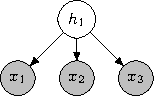
\includegraphics[width=0.95\textwidth,height=4cm,keepaspectratio]{figures/three-view.pdf} \\
      \includegraphics[width=0.95\textwidth,keepaspectratio]{figures/lhood.pdf}
    \end{figure}
    \vspace{-1cm}
  \begin{itemize}
    \item {\bf How can we apply the method of moments to consistently
      and efficiently estimate parameters for a general model family?}
  \end{itemize}
  }
\end{block}
\vfill

\begin{block}{Setup}
  \splitcolumn{%
    \begin{itemize}
      \item Assume discrete models with $k$ hidden and $d \ge k$
        observed values.
      \item Parameters and marginals can be represented as matrices
        and tensors.
      \item Presented in terms of infinite data and exact moments.
      \item Directed models are parameterized by their conditional
        probability tables.
      \item Undirected models are parameterized as a log-linear model,
        {\small
        \begin{align*}
        p(x) &= \exp(\sum_{\sC \in \sG} \theta^\top \phi(x_\sC, h_\sC) - A(\theta)).
        \end{align*}
        }
    \end{itemize}
 }{%
    \centering
    \begin{tikzpicture}
        % The model
        \point{start}{(0cm,0cm)}; %{pic cs:gen} -| mark)};
        % Matrices
        % - M12
        \node[scale=0.8] (m12) at ($(start) + (0.5cm,0.25cm)$) {\objw{3cm}{
          \begin{align*}
            M_{12} &\eqdef \Pr(x_1, x_2) \\
            {\color{blue} (M_{12})_{ij}} &\eqdef {\color{blue} \Pr(x_1 = i, x_2 = j)}
          \end{align*}
          }
        };
%        \point{m12c}{($(m12) + (1.5cm,0.75cm)$)};
         \tikzrect{m12r}{black,fill=white} {($(m12) + (3.2cm,0.75cm)$)}{1}{1};
         \tikzrect{m12ijr}{black,fill=blue}{($(m12) + (3.2cm,0.75cm)$)}{0.2}{0.2};
        % - M123
        \node[below=0.25cm of m12, scale=0.8] (m123) {\objw{3cm}{
          \begin{align*}
            M_{123} &\eqdef \Pr(x_1, x_2, x_3) \\
            {\color{blue} (M_{123})_{ijk}} &\eqdef {\color{blue} \Pr(x_1 = i, x_2 = j, x_3=k)}
          \end{align*}
          }
        };
%        \point{m123-c}{($(m123) + (1.75cm,0.75cm)$)};
        \tikzcube{m123r}{black,fill=white} {($(m123) + (3.2cm,0.75cm)$)}{1}{1}{1};
        \tikzcube{m123ijr}{black,fill=blue}{($(m123) + (3.2cm,0.75cm)$)}{0.2}{0.2}{0.2};

        % - O11
        \node[below=0.25cm of m123, scale=0.8] (o11) {\objw{3cm}{
          \begin{align*}
            \mOpp{1}{1} &\eqdef \Pr(x_1 \given h_1) \\
            {\color{DarkGreen} (\mOpp{1}{1})_{ij}} &\eqdef {\color{DarkGreen} \Pr(x_1 = i \given h_1 = j)}
          \end{align*}
          }
        };
%        \point{m123-c}{($(m123) + (1.75cm,0.75cm)$)};
        \tikzrect{o11r}{black,fill=white} {($(o11) + (3.2cm,0.75cm)$)}{1}{1};
        \tikzrect{o11ijr}{black,fill=DarkGreen}{($(o11) + (3.2cm,0.75cm)$)}{0.2}{0.2};
      \end{tikzpicture}
      \begin{tikzpicture}
        \point{stuff}{(2cm,0cm)};
        \drawbridge{(stuff)};
        \node[scale = 0.5, anchor=south] at (h1h2) {
          \begin{tabular}{r | l l}
            \diaghead{aaaaaa}{$h_2$}{$h_1$} &
            \thead{$0$} & \thead{$1$} \\ \hline 
            $0$ & \quad & \quad \\ 
            $1$ & \quad & \quad 
          \end{tabular}
        };
      \end{tikzpicture}
      \begin{tikzpicture}
        \point{stuff}{(2cm,0cm)};
        \drawubridge{(stuff)};
        \node[scale = 1.0, anchor=south] at (h1h2) {$\theta$};
      \end{tikzpicture}
  }
\end{block}
\vfill

\begin{block}{1. Bottlenecks}
  \splitcolumn{%
    \begin{itemize}
      \item A hidden variable $h$ is a {\bf bottleneck} if there exist three
        observed variables ({\bf views}) $x_1, x_2, x_3$ that are
        {\em conditionally independent} given $h$.
      \item We say a set of variables is {\em bottlenecked} if each
        variable is a bottleneck.
    \end{itemize}
  }{%
    \begin{itemize}
      \item \cite{anandkumar13tensor} provide an algorithm to estimate
        conditional moments $\Pr(x_i \given h)$ based on tensor
        eigendecomposition.
      \end{itemize}
  }
\end{block}
\vfill
\begin{block}{Limitations of bottlenecks}
  \splitcolumn{%
    \begin{itemize}
      \item Solving bottlenecks only provide conditional moments
        $\mOpp{1}{1} \eqdef \Pr(x_1 \given h_1)$. There are parameters
        that are not conditional moments. For example $\Pr(h_2 \given
        h_1)$ in the bridge model.
      \item {\bf An alternate approach:} fix the conditional moments;
        then the hidden marginals $Z_{12}$ and observed moments $M_{12}$
        are linearly related and can be solved.
      \item Main takeaway: Fixing conditional moments (learned using
        bottlenecks) simplifies learning other parameters.
    \end{itemize}
  }{%
  {
    \begin{figure}
    \centering
    \begin{tikzpicture}
    \point{mark}{(0,0)};
    \drawbridge{(mark)};
    \begin{pgfonlayer}{background}
    \draw[draw=black,fill=green!70,rounded corners,line width=1pt, dotted] 
                    ($(x1a.west) + (180:0.3cm)$) -- 
                    ($(h1.north) + (90:0.3cm)$) -- 
                    ($(x2a.east) + (0:0.3cm)$) -- 
                    ($(x2a.south) + (-90:0.3cm)$) -- 
                    ($(x1b.south) + (-90:0.3cm)$) -- 
                    ($(x1a.south) + (-90:0.3cm)$) -- 
                    cycle;
    \draw[dashed,-latex] (h1) -- (x2a);
    \end{pgfonlayer}
    \draw[-latex,DarkGreen] (h1) -- (x1a);
    \draw[-latex,DarkGreen] (h1) -- (x1b);

    \draw[-latex,DarkGreen,dashed] (h1) -- (x2a);

     \draw[-latex,DarkGreen] (h2) -- (x2a);
     \draw[-latex,DarkGreen] (h2) -- (x2b);
     \draw[-latex,DarkGreen,dashed] (h2) -- (x1b);

     \draw[-latex,red] (h1) -- (h2);
    \end{tikzpicture}
    \caption{The bridge model}
    \end{figure}
    }

    {\small
    \begin{align*}
      \underbrace{\Pr(x_1^b, x_2^a)}_{M_{12}} &= \sum_{h_1, h_2} 
      \underbrace{\Pr(x_1^b | h_1)}_{\mOpp{1}{1}}
      \underbrace{\Pr(x_2^a | h_2)}_{\mOpp{2}{2}}
      \underbrace{\Pr(h_1, h_2)}_{Z_{12}} \\
      M_{12} &= \mOpp{1}{1} Z_{12} \mOppt{2}{2} \\
      Z_{12} &= \mOppi{1}{1} M_{12} \mOppit{2}{2}
    \end{align*}
    }
  }
\end{block}


          }
        \end{minipage}
      \end{beamercolorbox}
    \end{column}

    %%%%%%%%%%%%%%%%%%%%%%%%%%%%%%%%%%%%%%%%%%%%%%%%%%%%%%%%%%%%%%%%%%%%%%%%%%%%%%%%%%%%%%
    % Column 2
    \begin{column}{.49\textwidth}
      \begin{beamercolorbox}[center,wd=\textwidth]{postercolumn}
        \begin{minipage}[T]{.95\textwidth} % tweaks the width, makes a new \textwidth
          \parbox[t][\columnheight]{\textwidth}{% must be some better way to set the the height, width and textwidth simultaneously
            % Since all columns are the same length, it is all nice and tidy.  You have to get the height empirically
            % ---------------------------------------------------------%
            % fill each column with content
            \begin{block}{Step 1: Finding Tensor Structure via Regression}
  \begin{itemize}
    \item {\bf Key Observation:} Regression on the powers of
        $(y,x)$ gives us the expected powers of the regression
        coefficients $\beta$. 
    \begin{columns}
      \begin{column}{0.65\textwidth}
  \begin{align*}
    y\tikzmark{regA} 
      &= \innerpp{\beta_h}{x} + \epsilon \\
      &= \mathmb{\ub{\innerp{\E[\beta_h]}{x}}_{\textrm{linear measurement}}} &&+ \mathmr{\ub{(\beta_h - \E[\beta_h])^T x + \epsilon}_{\textrm{noise}}} \\
    y^2 \tikzmark{regB}
      &= \left(\innerp{\beta_h}{x} + \epsilon\right)^2 && \\
      &= \mathmb{\innerpp{\ub{\E[\beta_h\tp{2}]}_{M_2}}{x\tp{2}}}
      &&+ \mathmg{\textrm{bias}_2} + \mathmr{\textrm{noise}_2} \\
    y^3 \tikzmark{regC}
    &= \mathmb{\innerpp{\ub{\E[\beta_h\tp{3}]}_{M_3}}{x\tp{3}}} &&+ \mathmg{\textrm{bias}_3} + \mathmr{\textrm{noise}_3}
  \end{align*}
    \end{column}
      \begin{column}{0.25\textwidth}
  \begin{tikzpicture}
    \point{mark}{(0,0)};
      \regressionA{($(mark) + (0,0cm)$)};
      \regressionB{($(mark) + (0,-2.5cm)$)};
      \regressionC{($(mark) + (0,-4.5cm)$)};
  \end{tikzpicture}
    \end{column}
  \end{columns}


\item $M_2$ and $M_3$ are both of rank $k$, so we can use low rank regression$^{3,4}$!
  \begin{align*}
    \hat M_2 
      &= \arg\min_{M} \sum_{(x,y)\in\mathcal{D}} 
        \left( y^2 - \innerp{M}{x\tp{2}} - \textrm{bias}_2\right)^2 
          + \lambda_2 \mathmb{\ub{\|M\|_{*}}_{\sum_i \sigma_i(M)}}\\
    \hat M_3 
      &= \arg\min_{M} \sum_{(x,y)\in\mathcal{D}} 
        \left( y^3 - \innerp{M}{x\tp{3}} - \textrm{bias}_3\right)^2 
        + \lambda_3 \|M\|_{*}
  \end{align*}
  \end{itemize}

  \footnotesize{%
  \hfill
    [3] Fazel, 2002; [4] Tomoika, Hayashi and Kashima, 2010
  }

\end{block}

\begin{block}{Step 2: Parameter Recovery via Tensor Factorization}
  \begin{itemize}
      \item $M_3$ has a low-rank tensor decomposition:
      $M_3 = \sum_{h=1}^k \pi_h \beta_h\tp{3}$
      \vspace{1ex}\\
      \begin{tikzpicture}[scale=1.5]
          \tensorfactorization{(0cm,0cm)};
      \end{tikzpicture}

    \item {\bf Key Observation:} If $\beta_h$ are orthogonal, they are eigenvectors$^{5}$; 
      $M_3(\beta_h,\beta_h) = \pi_{h} \beta_{h}$.
    \item In general, we can whiten $M_3$ first.
  \end{itemize}
  \footnotesize{%
  \hfill
  [5]: Anandkumar, Ge, Hsu, Kakade, Telgarksy, 2012.
  }

\end{block}

\begin{block}{Experiments}
  \begin{itemize}
      \item With finite samples, Spectral Experts seems to find parameters
        that sufficiently separate components that EM initialized with
        these parameters recovers true parameters more often than EM with random initializations.
  \item In this example, $y = \beta^T [ 1, t, t^4 ,t^7 ]^T + \epsilon$. $k = 3, d = 4, n = 10^5$,
  \begin{tikzpicture}
    \node (graphs) {%
      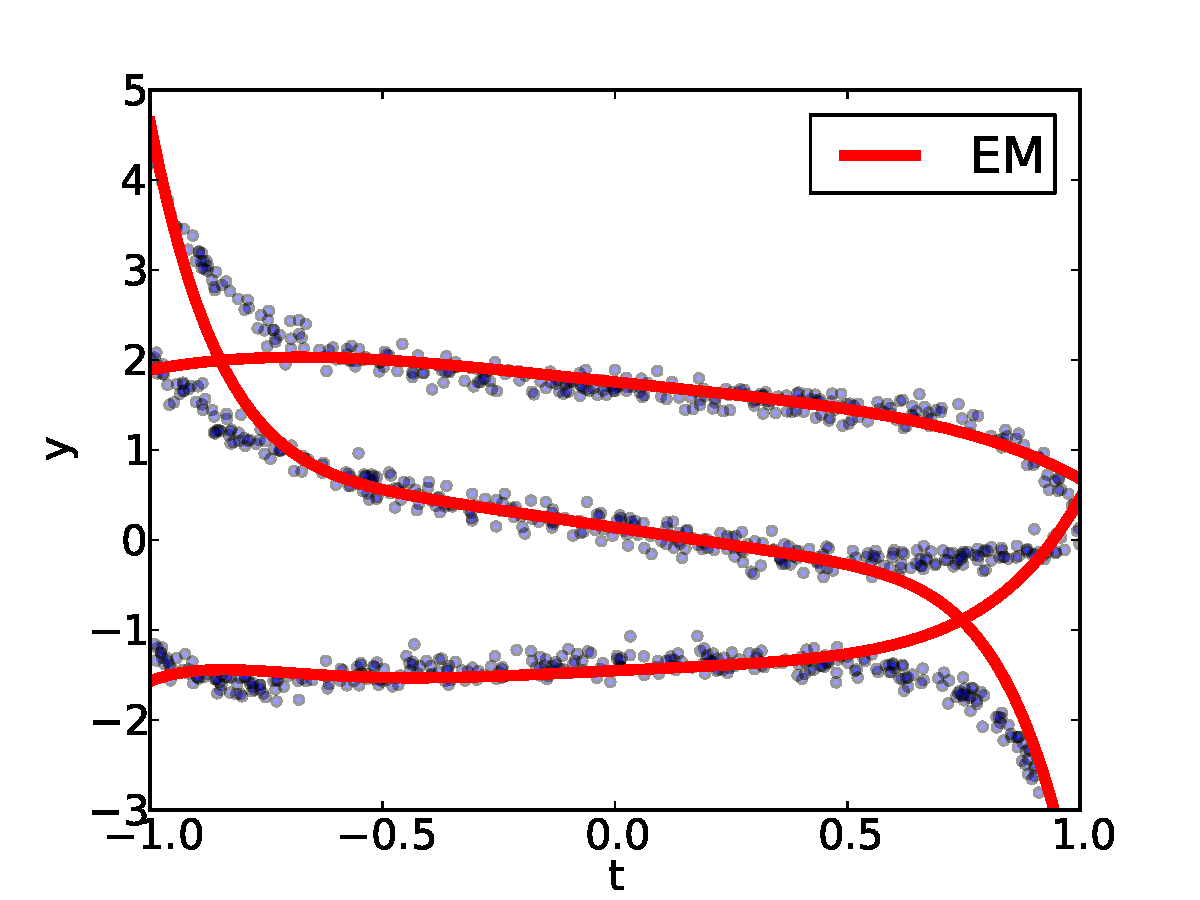
\includegraphics[width=0.3\textwidth,height=5cm,keepaspectratio]{figures/EM-1833.pdf}
      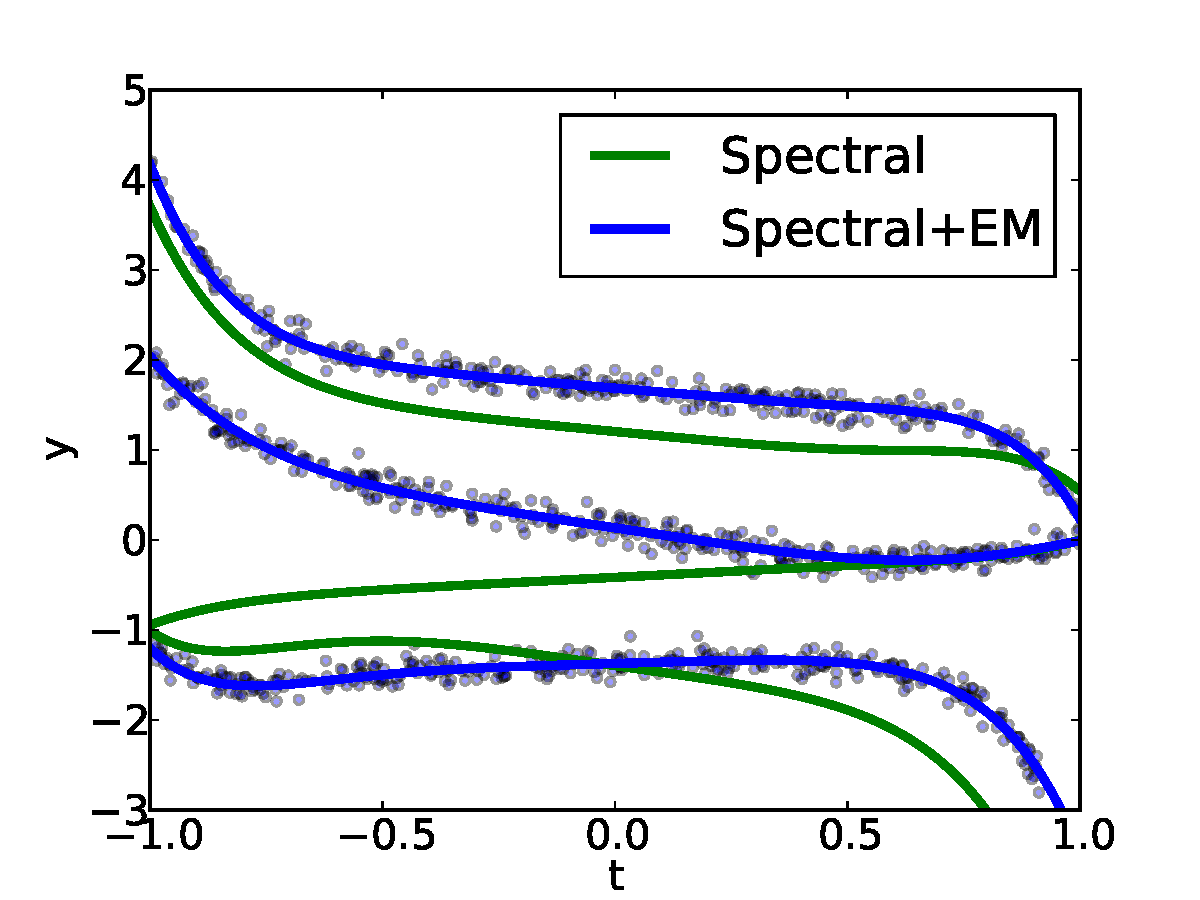
\includegraphics[width=0.3\textwidth,height=5cm,keepaspectratio]{figures/Spectral-Spectral+EM-1833.pdf}
      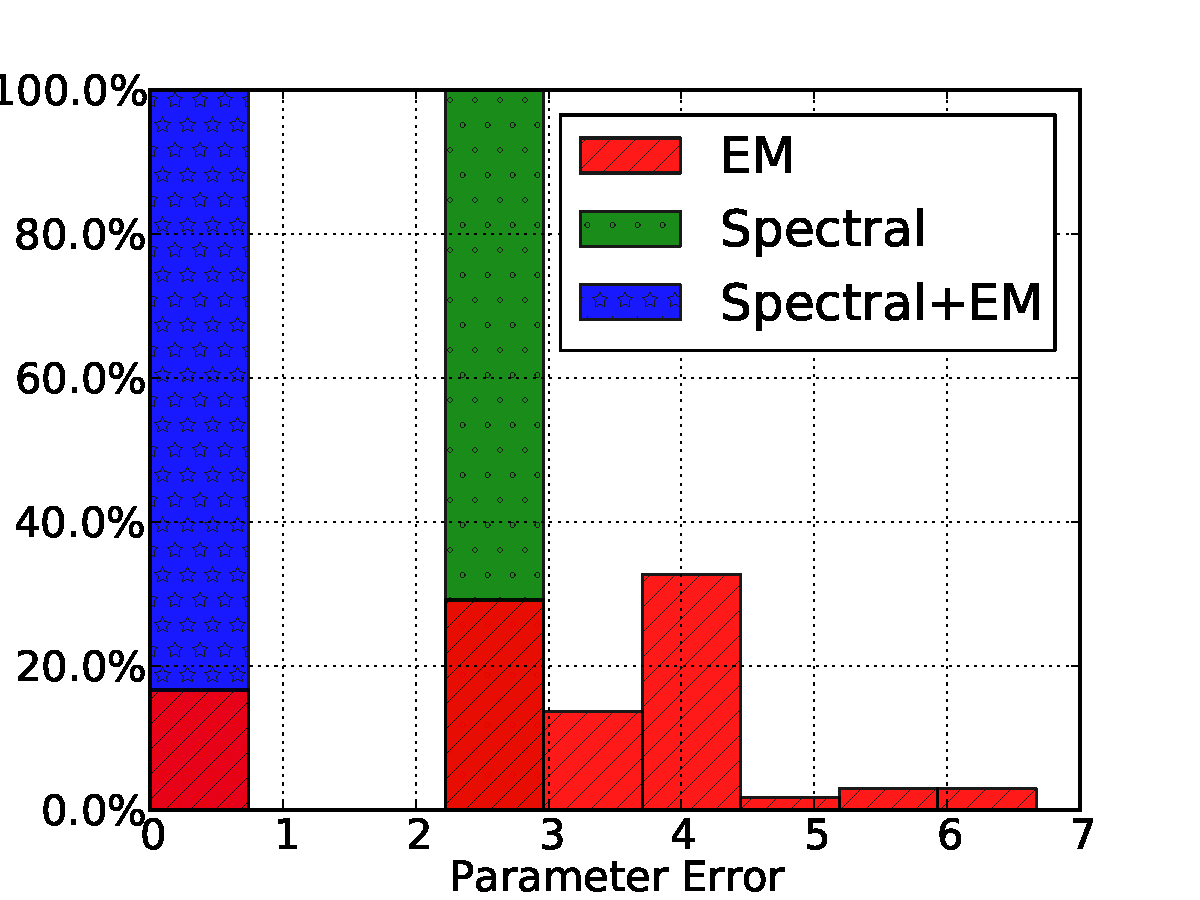
\includegraphics[width=0.3\textwidth,height=5cm,keepaspectratio]{figures/EM-Spectral-Spectral+EM-hist.pdf}
      };
  \end{tikzpicture}
  \item Below are parameter errors averaged over 10 initializations on
    10 different simulated datasets with the specified parameter
    configurations,
    \begin{tikzpicture}
      \node (exp1) {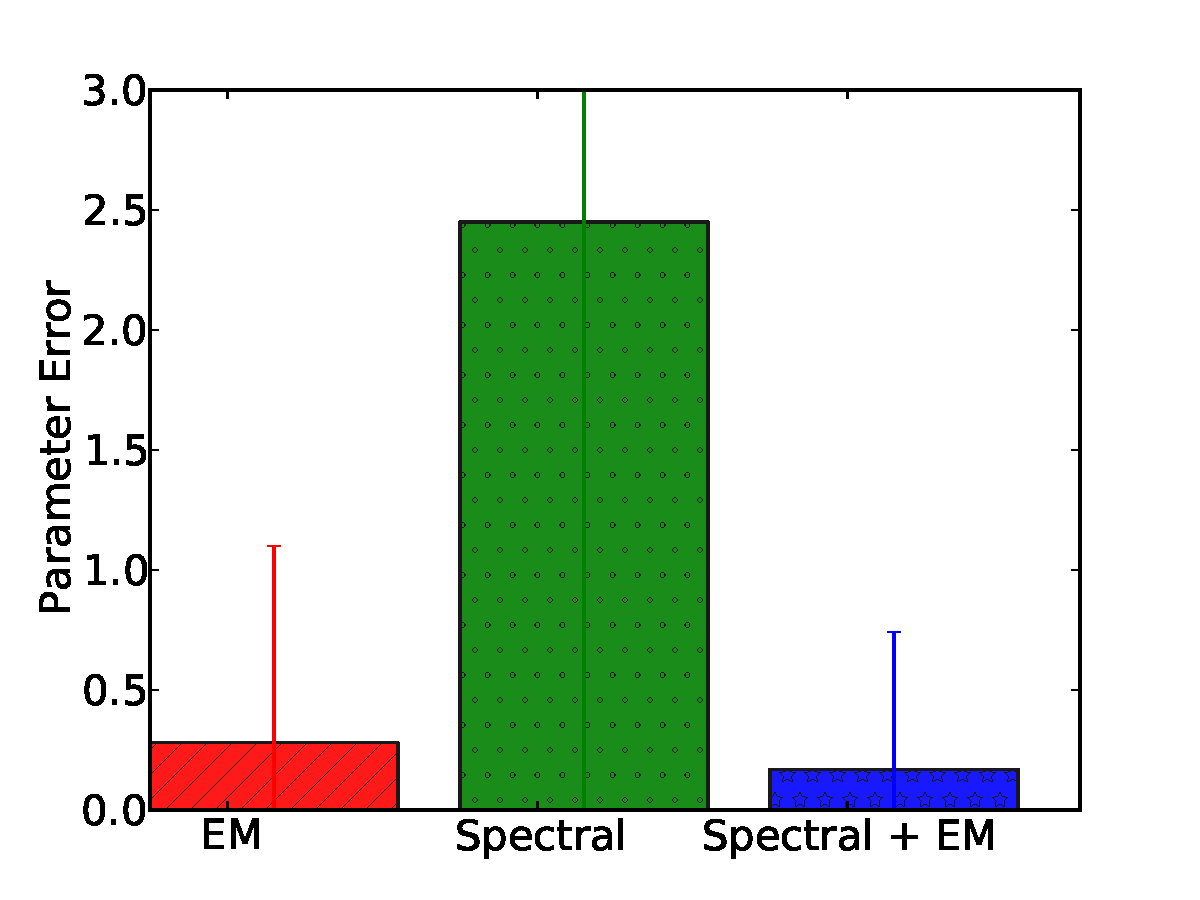
\includegraphics[width=0.2\textwidth]{figures/err-hist-0.pdf}};
      \node[scale=0.8,below=-0.2cm of exp1] {$d=4, k=2$};
      \node[right=0cm of exp1] (exp2) {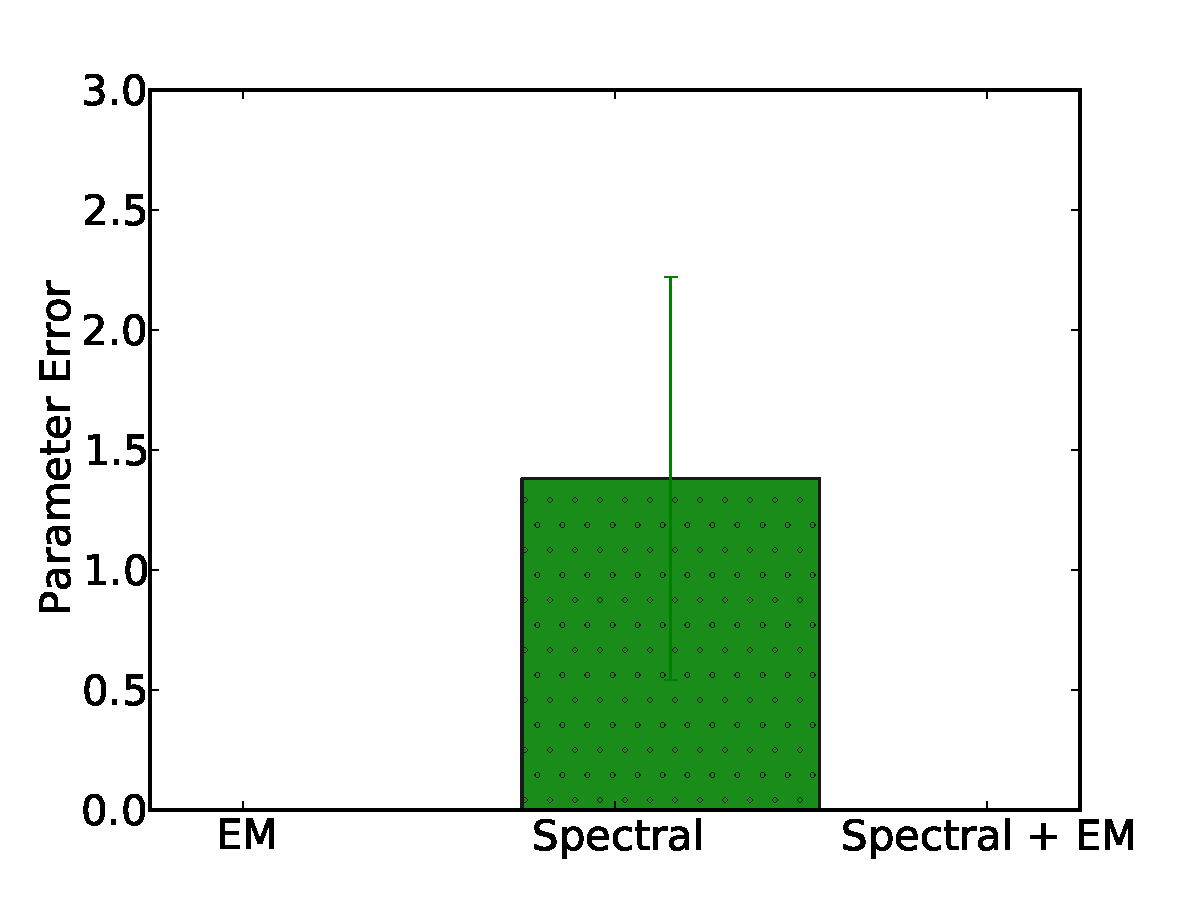
\includegraphics[width=0.2\textwidth]{figures/err-hist-1.pdf}};
      \node[scale=0.8,below=-0.2cm of exp2] {$d=5, k=2$};
      \node[right=0cm of exp2] (exp3) {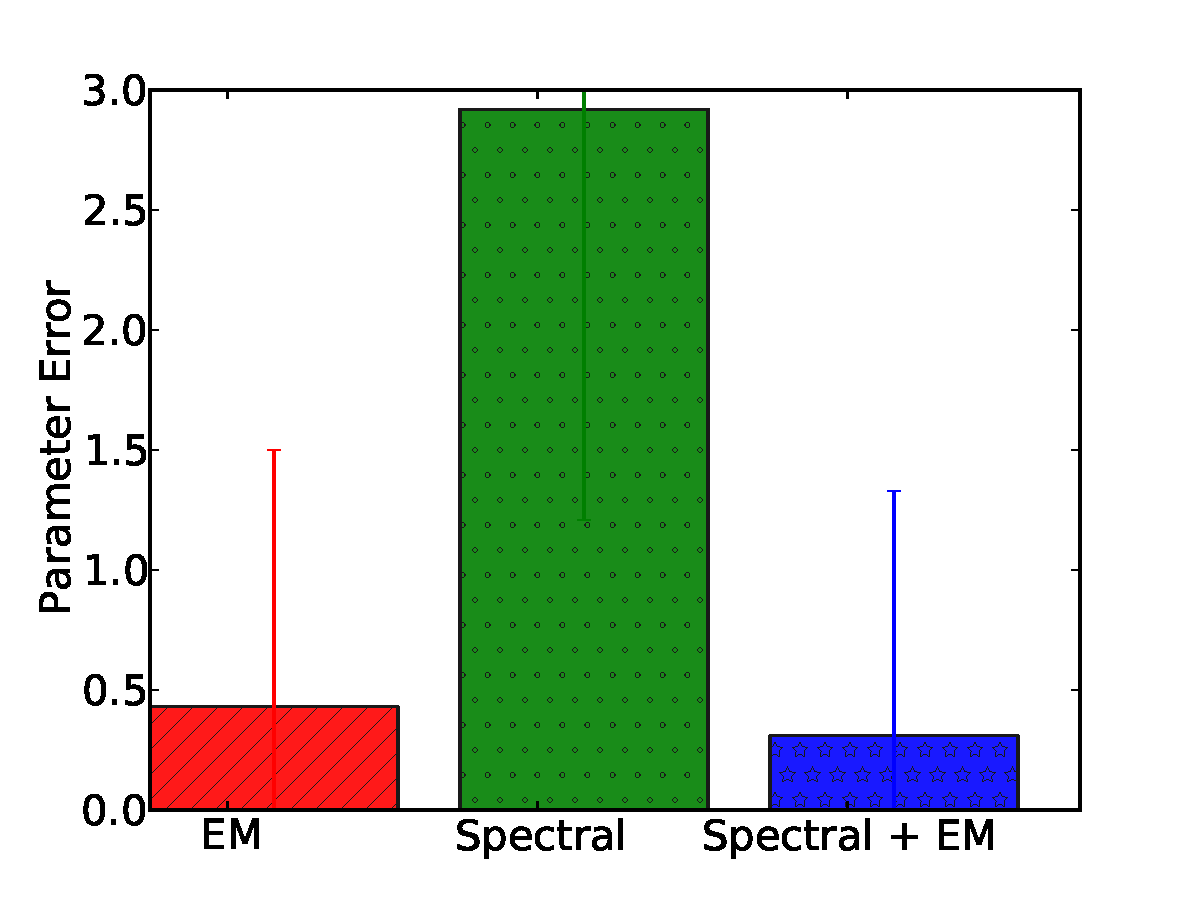
\includegraphics[width=0.2\textwidth]{figures/err-hist-2.pdf}};
      \node[scale=0.8,below=-0.2cm of exp3] {$d=5, k=3$};
      \node[right=0cm of exp3] (exp4) {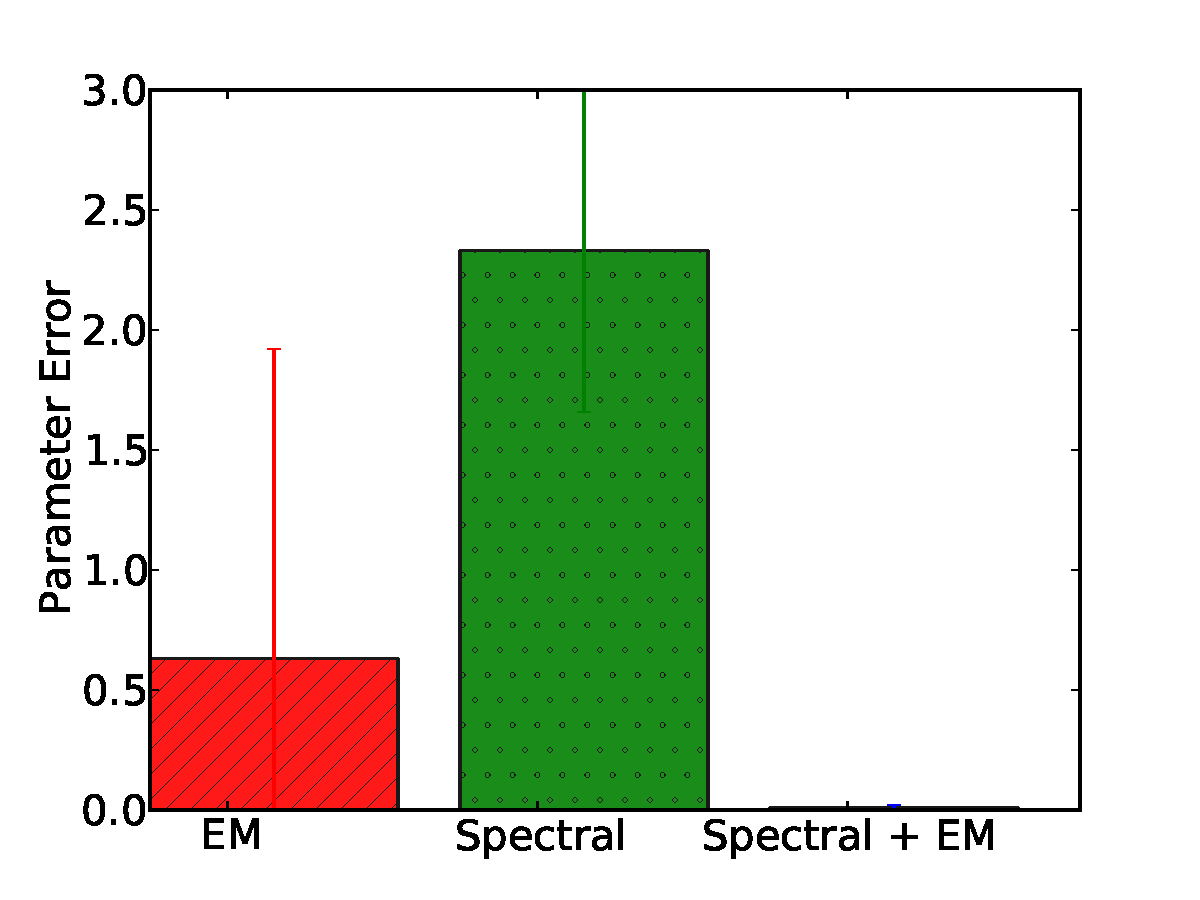
\includegraphics[width=0.2\textwidth]{figures/err-hist-3.pdf}};
      \node[scale=0.8,below=-0.2cm of exp4] {$d=6, k=2$};
    \end{tikzpicture}

  \item {\bf Log-likelihood cartoon:} It seems that our parameter estimates fall in the right basin of attraction for EM.\\
      \begin{tikzpicture}
        \point{mark}{(0,0)}
        % x, y
        \llhood{4cm}{0};

        \node[scale=0.3,circle,fill=red] at (em2) {};
        \node at ($(em2) + (0.7cm,0)$) {$\mathmr{\hat\theta_{\textrm{EM}}}$};
        \draw[-latex,smooth,line width=1pt,red] ($(em2-start) + (+0.1cm,+0.05cm)$) -- ($(em2) + (+0.15cm,0.00cm)$);
        %\draw[dashed,red,line width=0.7pt] ($(em2)-(3.5cm,0)$) -- ($(em2)+(0.5cm,0)$);

    %    \draw<3>[latex-latex,DarkGreen,line width=1pt,dashed] ($(mle) + (-1.2cm,0.8cm)$) -- node[above]{$\mathmg{\epsilon}$} ($(mle) + (+1.2cm,0.8cm)$);
        \node[scale=0.3,circle,fill=DarkGreen] at (spec) {};
        \node at ($(spec) + (0.6cm,0.3cm)$) {$\mathmg{\hat\theta_{\textrm{spec}}}$};
        %\draw[dashed,DarkGreen,line width=0.7pt] ($(spec)-(0.5cm,0)$) -- ($(spec)+(3.5cm,0)$);

        \draw[-latex,smooth,line width=1pt,DarkGreen] ($(spec) + (-0.1cm,+0.05cm)$) -- ($(mle) + (-0.30cm,+0.10cm)$);
        \node[scale=0.3,circle,fill=blue] at (mle) {};
        \node[anchor=west] at ($(mle) + (0.2cm,0)$) {$\mathmb{\hat\theta}_{\textrm{spec + EM}}$};

        %\draw[dashed,blue,line width=0.7pt] ($(mle)-(0.4cm,0)$) -- ($(mle)+(0.4cm,0)$);
      \end{tikzpicture}
  \end{itemize}
  \vspace{-1ex}

\end{block}

\begin{block}{Future Work}
  \begin{itemize}
    \item How can we handle other discriminative models?
      \begin{itemize}
          \item Non-linear link functions (hidden variable logistic regression).
          \item Dependencies between $h$ and $x$ (mixture of experts).
      \end{itemize}
  \end{itemize}

\end{block}


\vfill


          }
          % ---------------------------------------------------------%
          % end the column
        \end{minipage}
      \end{beamercolorbox}
    \end{column}
    % ---------------------------------------------------------%
    % end the column
  \end{columns}
  \vskip2ex
\end{frame}

\end{document}

